%!TEX root = ../main.tex

\chapter{Discussione}\label{chp:discussion}



\begin{table}[!h]
    \centering
    \renewcommand{\arraystretch}{2}
    \begin{tabular}{|c|c|c|c|c|c|} % chktex-file 44
        \hline % chktex-file 44
        \textbf{Modello} & \textbf{Struttura} & \textbf{Codifica} & \textbf{Kernel} & \textbf{Dataset} & \textbf{Funzione costo}\\ 
        \hline\hline % chktex-file 44
        \hyperref[sec:DeepSEA]{\textsl{DeepSEA}} & & One-hot Encoding & \acs{PWM} & & \textsl{Binary Cross Entropy} \\ 
        % 
        \hyperref[sec:Basset]{\textsl{Basset}} & & One-hot Encoding & \acs{PWM} & & \textsl{Binary Cross Entropy} \\ 
        % 
        \hyperref[sec:DeepSATA]{\textsl{DeepSATA}} & & One-hot Encoding & & &  \\ 
        \hline
    \end{tabular}
    \renewcommand{\arraystretch}{1}
\end{table}




\begin{table}[!h]
    \centering
    \renewcommand{\arraystretch}{2}
    \begin{tabular}{|c|c|c|c|c|c|} % chktex-file 44
        \hline % chktex-file 44
        \textbf{Modello} & \textbf{Topi} & \textbf{Maiali} & \textbf{Bovini} & \textbf{Umani} & \textbf{Polli}\\ 
        \hline\hline % chktex-file 44
        \hyperref[sec:DeepSEA]{\textsl{DeepSEA}} & 0.796 & 0.775 & 0.769 & 0.755 & 0.736 \\ 
        % 
        \hyperref[sec:Basset]{\textsl{Basset}} & 0.778 & 0.719 & 0.768 & 0.717 & 0.722 \\ 
        % 
        \hyperref[sec:DeepSATA]{\textsl{DeepSATA}} & 0.854 & 0.779 & 0.772 & 0.759 & 0.744 \\ 
        \hline
    \end{tabular}
    \renewcommand{\arraystretch}{1}
\end{table}

\begin{figure}[!b]
    \centering
    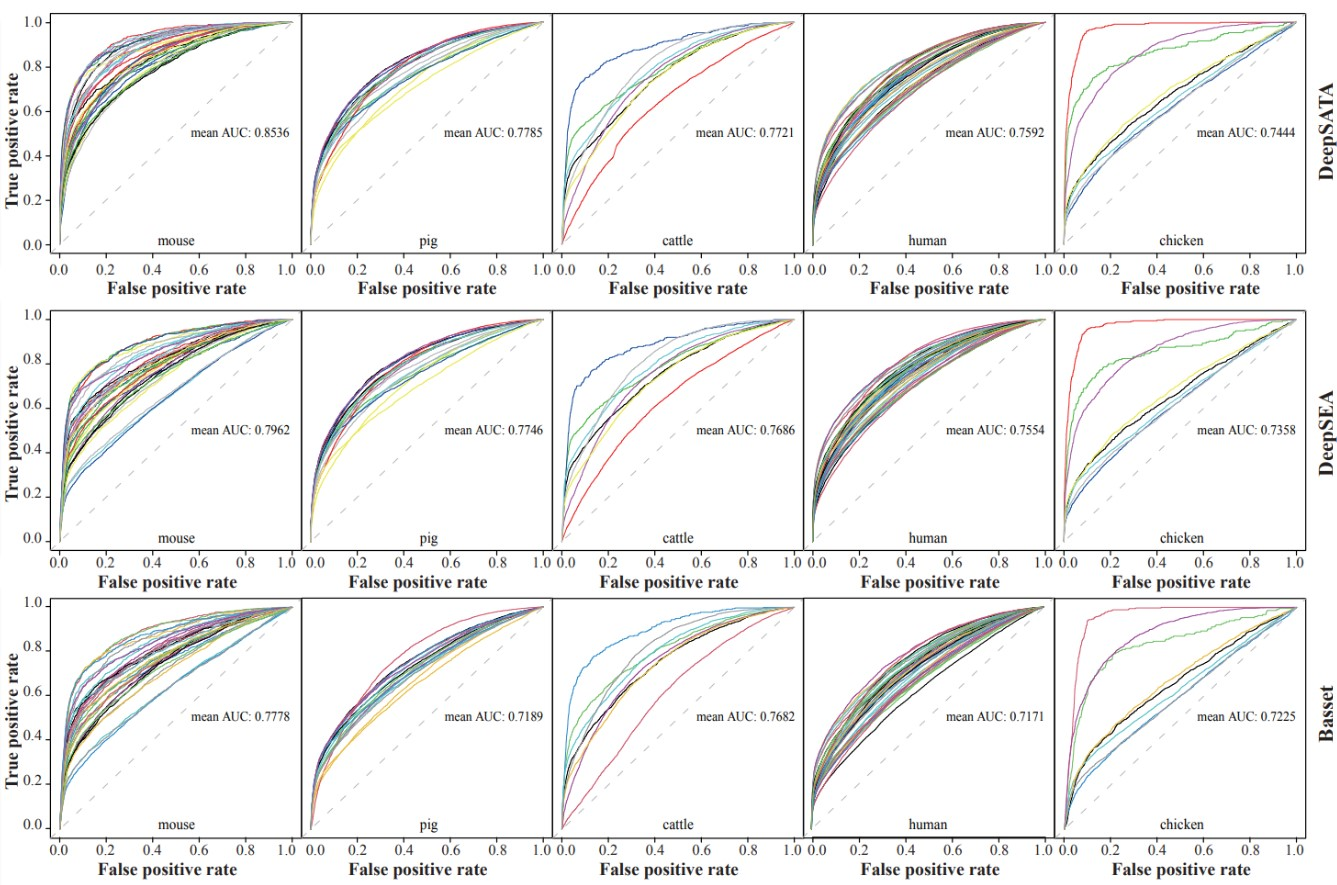
\includegraphics[width=1\textwidth]{assets/imgs/comparison.jpg}
    \caption[Confronto delle prestazioni predittive dei tre tool su diverse specie animali.]{Confronto delle prestazioni predittive dei tre tool su diverse specie animali.}\label{fig:comparison}
\end{figure}

\todo{Tabella che specifica e riassume per ogni tool encoding, dataset etc}
\todo{riassume quanto analizzato prima, riporta i risultati del paper piu recente in modo da avere un momento in cui riassumo la situa}
\todo{Sperimentalmente, per risorse a disposizione, per il confronto ci si basa sui risultati dell'ultimo paper}
